\documentclass{article}

\usepackage{graphicx}
\usepackage{tikz}
\usepackage{tikzsymbols}
\usetikzlibrary{calc,patterns,shapes.geometric}
\pagestyle{empty}
\usepackage[margin=0pt]{geometry}
\geometry{papersize={14in,12in}}

\def\centerarc[#1](#2)(#3:#4:#5){\draw[#1] ($(#2)+({#5*cos(#3)},{#5*sin(#3)})$) arc (#3:#4:#5);}

\begin{document}
	\begin{figure}
		\centering
		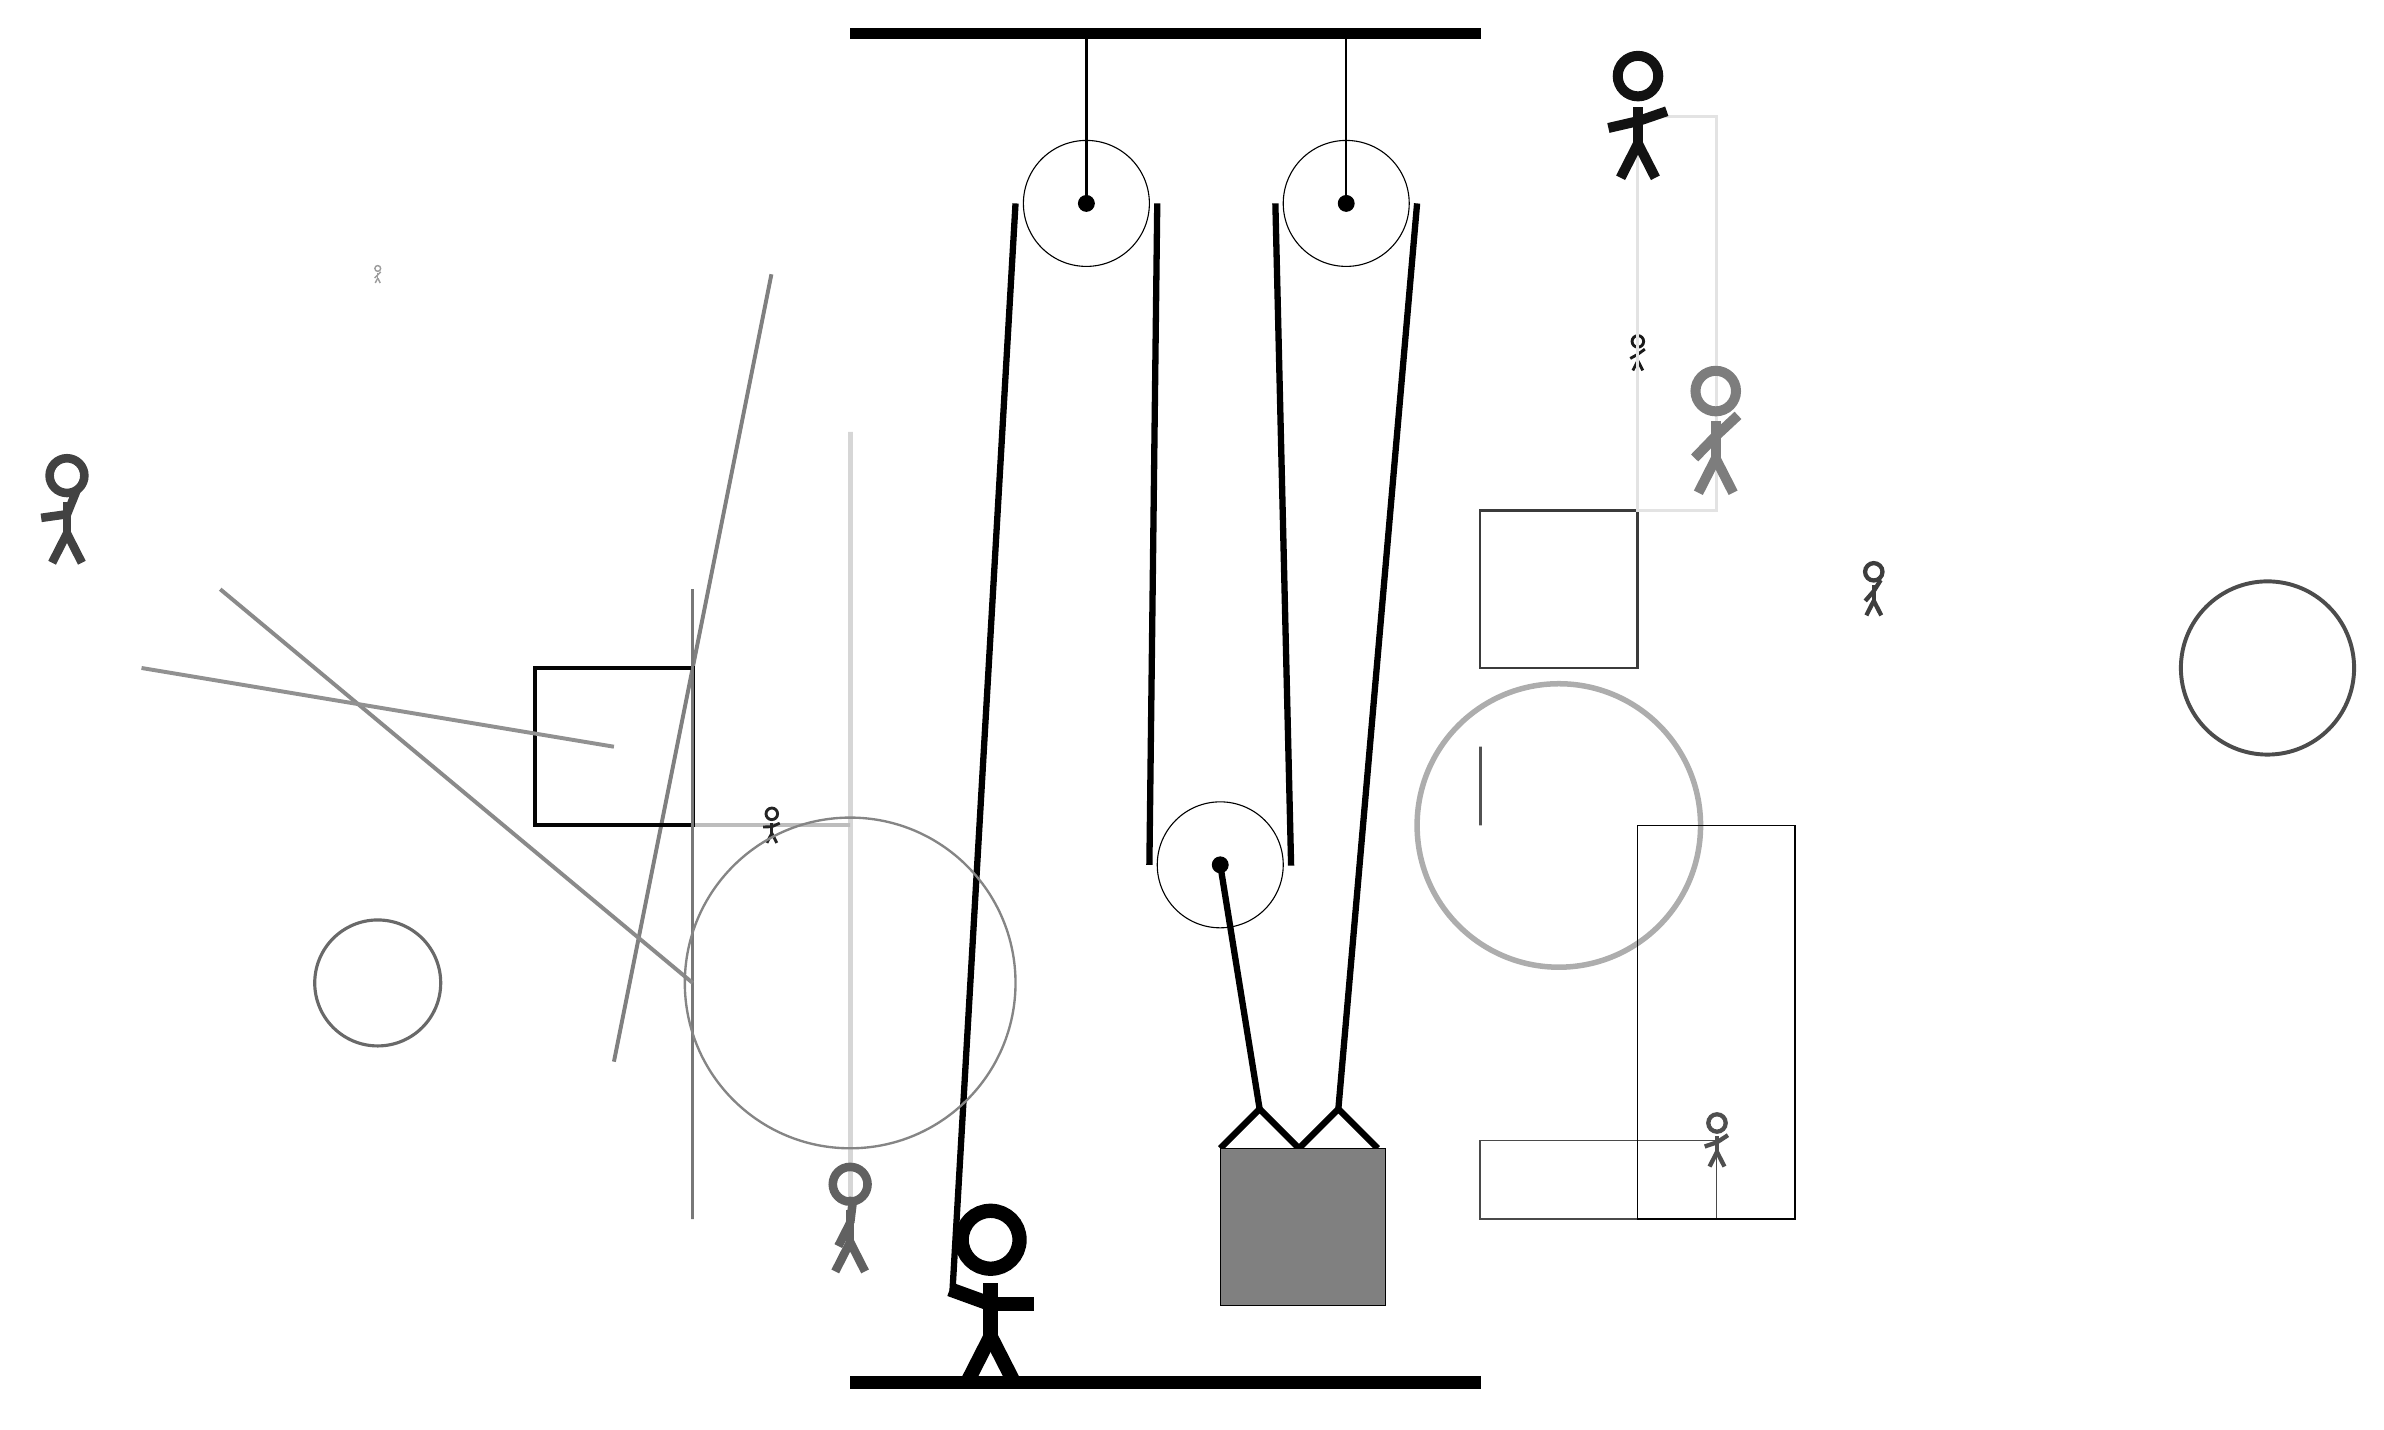
\begin{tikzpicture}
			%%%%% START %%%%%
			
			\draw[fill=black] (-2, 14) rectangle (6, 14.125);
			
			\draw (1, 11.9) circle (0.8);
			\draw[fill=black] (1, 11.9) circle (0.1);
			\draw[thick] (1, 11.9) -- (1, 14);
			
			\draw (4.3, 11.9) circle (0.8);
			\draw[fill=black] (4.3, 11.9) circle (0.1);
			\draw[thick] (4.3, 11.9) -- (4.3, 14);
			
			\draw (2.7, 3.5) circle (0.8);
			\draw[fill=black] (2.7, 3.5) circle (0.1);
			
			\draw[line width=0.8mm]  (2.7, -0.1) -- (3.2, 0.4) -- (3.7, -0.1) -- (4.2, 0.4) -- (4.7, -0.1);
			\draw[fill=black!50] (2.7, -0.1) rectangle (4.8, -2.1);
			
			\draw[line width=0.8mm](-0.7, -1.9) -- (0.1, 11.9);
			\centerarc[line width=0.8mm](1, 11.9)(0:180:0.9);
			\draw[line width=0.8mm](1.9, 11.9) -- (1.8, 3.5);
			\centerarc[line width=0.8mm](2.7, 3.5)(180:370:0.9);
			\draw[line width=0.8mm] (3.6, 3.49) -- (3.4, 11.9);
			\centerarc[line width=0.8mm](4.3, 11.9)(0:180:0.9);
			\draw[line width=0.8mm](4.2, 0.4) -- (5.2, 11.9);
			\draw[line width=0.8mm] (3.2, 0.4) -- (2.7, 3.5);
			
			\node at (-0.2, -2) {\Strichmaxerl[10][-20][0]};
			
			\draw[line width=0.6mm, color=black!16] (-2, -1) rectangle (-2, 9);
			
			\draw[line width=0.5mm, color=black!50](-3, 11) -- (-5, 1);
			\node[line width=0.6mm, color=black!90] at (8, 10) {\Strichmaxerl[2][29][36]};
			\draw [line width=0.5mm, color=black!70](16, 6) circle (1.1);
			\draw[line width=0.2mm, color=black!71] (6, 0) rectangle (9, -1);
			\draw[line width=0.3mm, color=black!77] (8, 8) rectangle (6, 6);
			\node[line width=0.5mm, color=black!74] at (-12, 8) {\Strichmaxerl[6][8][68]};
			\draw [line width=0.7mm, color=black!32](7, 4) circle (1.8);
			\draw[line width=0.4mm, color=black!11] (8, 8) rectangle (9, 13);
			
			\node[line width=0.6mm, color=black!69] at (9, 0) {\Strichmaxerl[3][19][33]};
			\draw[line width=0.5mm, color=black!26] (-2, 4) rectangle (-6, 4);
			
			\draw[line width=0.5mm, color=black!98] (-4, 4) rectangle (-6, 6);
			\draw[line width=0.4mm, color=black!53] (-4, -1) rectangle (-4, 7);
			
			\node[line width=0.7mm, color=black!86] at (-3, 4) {\Strichmaxerl[2][2][24]};
			\draw [line width=0.4mm, color=black!59](-8, 2) circle (0.8);
			\node[line width=0.7mm, color=black!51] at (9, 9) {\Strichmaxerl[7][46][43]};
			
			\draw[line width=0.5mm, color=black!46](-4, 2) -- (-10, 7);
			\node[line width=0.2mm, color=black!39] at (-8, 11) {\Strichmaxerl[1][44][45]};
			\draw[line width=0.5mm, color=black!43](-5, 5) -- (-11, 6);
			\node[line width=0.6mm, color=black!62] at (-2, -1) {\Strichmaxerl[6][63][83]};
			\draw[line width=0.2mm, color=black!99] (8, 4) rectangle (10, -1);
			
			\draw [line width=0.3mm, color=black!48](-2, 2) circle (2.1);
			
			\node[line width=0.4mm, color=black!76] at (11, 7) {\Strichmaxerl[3][49][58]};
			\node[line width=0.2mm, color=black!93] at (8, 13) {\Strichmaxerl[7][13][19]};
			\draw[line width=0.4mm, color=black!68] (6, 5) rectangle (6, 4);
			
			
			\draw[fill=black] (-2, -3) rectangle (6, -3.15);
			
			%%%%% END %%%%%
		\end{tikzpicture}
	\end{figure}	
\end{document}